\begin{figure*}[t]
  \begin{subfigure}[b]{0.8\textwidth}
  \centering
    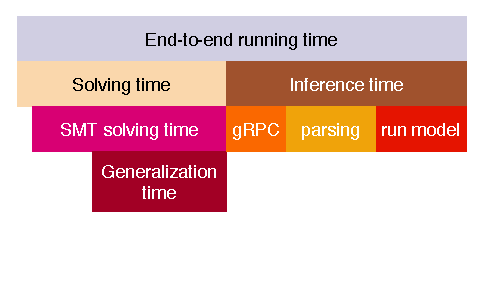
\includegraphics[width=0.6\textwidth]{figures/doping-flame.pdf}
    \caption{\mbox{Runtime~dist.~of~\dpy.}}
    \label{subfig:dpy_vs_spc_ind_gen}
	\end{subfigure}
  \centering
  \begin{subfigure}[b]{0.24\textwidth}
  \centering
    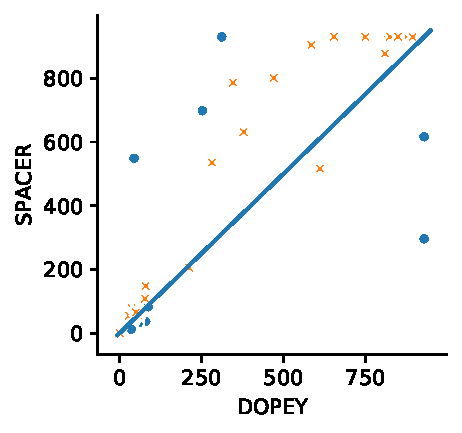
\includegraphics[width=0.99\textwidth]{figures/res-dpy_vs_spc_total.pdf}
    \caption{Solving + infer. time.}
    \label{subfig:dpy_vs_spc_total}
	\end{subfigure}
  \begin{subfigure}[b]{0.24\textwidth}
  \centering
    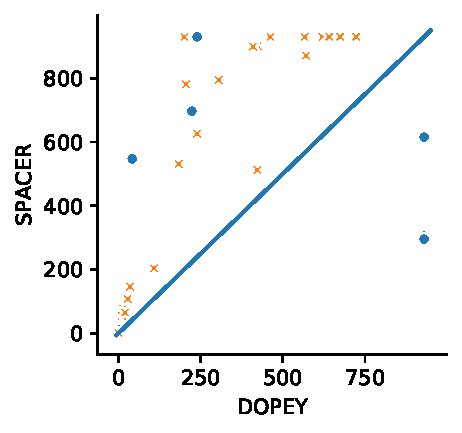
\includegraphics[width=0.99\textwidth]{figures/res-dpy_vs_spc_total_inside.pdf}
    \caption{Solving time.\linebreak}
    \label{subfig:dpy_vs_spc_total_sub}
  \end{subfigure}
  \begin{subfigure}[b]{0.24\textwidth}
  \centering
    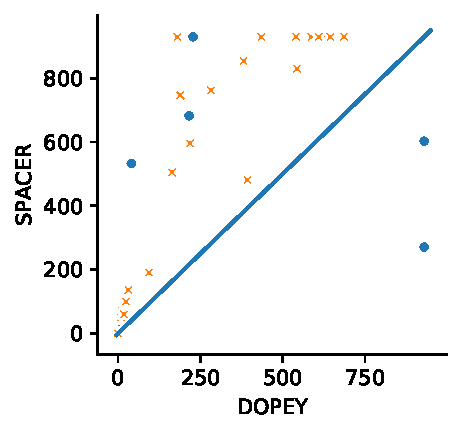
\includegraphics[width=0.99\textwidth]{figures/res-dpy_vs_spc_smt_solver.pdf}
    \caption{SMT-solving time.\linebreak}
    \label{subfig:dpy_vs_spc_smt}
	\end{subfigure}
  \begin{subfigure}[b]{0.24\textwidth}
  \centering
    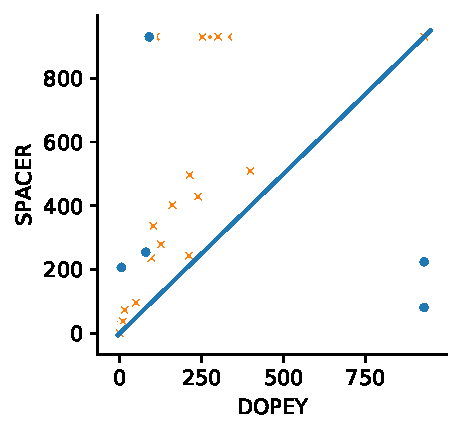
\includegraphics[width=0.99\textwidth]{figures/res-dpy_vs_spc_indgen.pdf}
    \caption{Generalization time.}
    \label{subfig:dpy_vs_spc_ind_gen_sub}
	\end{subfigure}

	\caption{Comparing \dpy's and \spc's running time, where blue dot ({\color{blue}\textbullet}) indicates an instance with unsafe property,  orange cross ({\color{orange}\textbf{x}}) indicates an instance with safe property, top (right) most place are instances \spc (\dpy) timed out.}
% 	\xs{remove the lengend, get rid of square shapes in the plot} }
  \label{fig:dpy_vs_spc}
\end{figure*}


